\chapter{Algoritmos para exploración en grafos}\label{grafos}

\section{Enunciado}\label{grafos-enunciado}

\textbf{“La Maleta de Luke” (El Profesor Layton y la Caja de Pandora, Nintendo DS)}

Disponemos de una maleta modelada mediante un rectángulo de $6$ casillas de alto por $9$ de ancho, y un conjunto de 8 objetos que hay que introducir en la maleta, cada uno modelado mediante un rectángulo de $5\times5$ casillas.
De esas $5\times5$ casillas que puede ocupar un objeto, sólo unas cuantas serán usadas para representarlo, dejando el resto de casillas como invisibles.
Un ejemplo de objetos a incluir son (sólo se visualizan las casillas útiles de cada objeto):

\begin{figure}[h]
\begin{center}
\tikzset{every picture/.style={line width=0.75pt}} %set default line width to 0.75pt

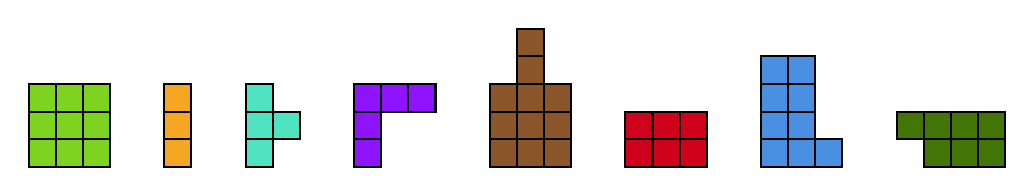
\begin{tikzpicture}[x=1pt,y=1pt,yscale=-1,xscale=1]
%uncomment if require: \path (0,235); %set diagram left start at 0, and has height of 235

%Shape: Rectangle [id:dp9777322586147241]
\draw  [color={rgb, 255:red, 0; green, 0; blue, 0 }  ,draw opacity=1 ][fill={rgb, 255:red, 126; green, 211; blue, 33 }  ,fill opacity=1 ][line width=0.75]  (180.15,50.04) -- (189.95,50.04) -- (189.95,60.04) -- (180.15,60.04) -- cycle ;
%Shape: Rectangle [id:dp5643921503512281]
\draw  [color={rgb, 255:red, 0; green, 0; blue, 0 }  ,draw opacity=1 ][fill={rgb, 255:red, 126; green, 211; blue, 33 }  ,fill opacity=1 ][line width=0.75]  (189.95,50.04) -- (199.75,50.04) -- (199.75,60.04) -- (189.95,60.04) -- cycle ;
%Shape: Rectangle [id:dp2656365377183654]
\draw  [color={rgb, 255:red, 0; green, 0; blue, 0 }  ,draw opacity=1 ][fill={rgb, 255:red, 126; green, 211; blue, 33 }  ,fill opacity=1 ][line width=0.75]  (180.15,60.04) -- (189.95,60.04) -- (189.95,70.04) -- (180.15,70.04) -- cycle ;
%Shape: Rectangle [id:dp3442854146601232]
\draw  [color={rgb, 255:red, 0; green, 0; blue, 0 }  ,draw opacity=1 ][fill={rgb, 255:red, 126; green, 211; blue, 33 }  ,fill opacity=1 ][line width=0.75]  (189.95,60.04) -- (199.75,60.04) -- (199.75,70.04) -- (189.95,70.04) -- cycle ;
%Shape: Rectangle [id:dp026943086469769284]
\draw  [color={rgb, 255:red, 0; green, 0; blue, 0 }  ,draw opacity=1 ][fill={rgb, 255:red, 126; green, 211; blue, 33 }  ,fill opacity=1 ][line width=0.75]  (199.75,50.04) -- (209.55,50.04) -- (209.55,60.04) -- (199.75,60.04) -- cycle ;
%Shape: Rectangle [id:dp24178310152356564]
\draw  [color={rgb, 255:red, 0; green, 0; blue, 0 }  ,draw opacity=1 ][fill={rgb, 255:red, 126; green, 211; blue, 33 }  ,fill opacity=1 ][line width=0.75]  (199.75,60.04) -- (209.55,60.04) -- (209.55,70.04) -- (199.75,70.04) -- cycle ;
%Shape: Rectangle [id:dp8978302733140608]
\draw  [color={rgb, 255:red, 0; green, 0; blue, 0 }  ,draw opacity=1 ][fill={rgb, 255:red, 126; green, 211; blue, 33 }  ,fill opacity=1 ][line width=0.75]  (199.75,70.04) -- (209.55,70.04) -- (209.55,80.04) -- (199.75,80.04) -- cycle ;
%Shape: Rectangle [id:dp9781999160020896]
\draw  [color={rgb, 255:red, 0; green, 0; blue, 0 }  ,draw opacity=1 ][fill={rgb, 255:red, 126; green, 211; blue, 33 }  ,fill opacity=1 ][line width=0.75]  (189.95,70.04) -- (199.75,70.04) -- (199.75,80.04) -- (189.95,80.04) -- cycle ;
%Shape: Rectangle [id:dp9948264741762237]
\draw  [color={rgb, 255:red, 0; green, 0; blue, 0 }  ,draw opacity=1 ][fill={rgb, 255:red, 126; green, 211; blue, 33 }  ,fill opacity=1 ][line width=0.75]  (180.15,70.04) -- (189.95,70.04) -- (189.95,80.04) -- (180.15,80.04) -- cycle ;
%Shape: Rectangle [id:dp7670141233033437]
\draw  [color={rgb, 255:red, 0; green, 0; blue, 0 }  ,draw opacity=1 ][fill={rgb, 255:red, 245; green, 166; blue, 35 }  ,fill opacity=1 ][line width=0.75]  (229.15,50.04) -- (238.95,50.04) -- (238.95,60.04) -- (229.15,60.04) -- cycle ;
%Shape: Rectangle [id:dp04088026261938915]
\draw  [color={rgb, 255:red, 0; green, 0; blue, 0 }  ,draw opacity=1 ][fill={rgb, 255:red, 245; green, 166; blue, 35 }  ,fill opacity=1 ][line width=0.75]  (229.15,60.04) -- (238.95,60.04) -- (238.95,70.04) -- (229.15,70.04) -- cycle ;
%Shape: Rectangle [id:dp23910333841895082]
\draw  [color={rgb, 255:red, 0; green, 0; blue, 0 }  ,draw opacity=1 ][fill={rgb, 255:red, 245; green, 166; blue, 35 }  ,fill opacity=1 ][line width=0.75]  (229.15,70.04) -- (238.95,70.04) -- (238.95,80.04) -- (229.15,80.04) -- cycle ;
%Shape: Rectangle [id:dp5479449658889934]
\draw  [color={rgb, 255:red, 0; green, 0; blue, 0 }  ,draw opacity=1 ][fill={rgb, 255:red, 80; green, 227; blue, 194 }  ,fill opacity=1 ][line width=0.75]  (258.55,70.04) -- (268.35,70.04) -- (268.35,80.04) -- (258.55,80.04) -- cycle ;
%Shape: Rectangle [id:dp24900658665942066]
\draw  [color={rgb, 255:red, 0; green, 0; blue, 0 }  ,draw opacity=1 ][fill={rgb, 255:red, 80; green, 227; blue, 194 }  ,fill opacity=1 ][line width=0.75]  (258.55,50.04) -- (268.35,50.04) -- (268.35,60.04) -- (258.55,60.04) -- cycle ;
%Shape: Rectangle [id:dp9051424246072522]
\draw  [color={rgb, 255:red, 0; green, 0; blue, 0 }  ,draw opacity=1 ][fill={rgb, 255:red, 80; green, 227; blue, 194 }  ,fill opacity=1 ][line width=0.75]  (258.55,60.04) -- (268.35,60.04) -- (268.35,70.04) -- (258.55,70.04) -- cycle ;
%Shape: Rectangle [id:dp20877566400813574]
\draw  [color={rgb, 255:red, 0; green, 0; blue, 0 }  ,draw opacity=1 ][fill={rgb, 255:red, 80; green, 227; blue, 194 }  ,fill opacity=1 ][line width=0.75]  (268.35,60.04) -- (278.15,60.04) -- (278.15,70.04) -- (268.35,70.04) -- cycle ;
%Shape: Rectangle [id:dp7463070383085549]
\draw  [color={rgb, 255:red, 0; green, 0; blue, 0 }  ,draw opacity=1 ][fill={rgb, 255:red, 144; green, 19; blue, 254 }  ,fill opacity=1 ][line width=0.75]  (297.75,60.04) -- (307.55,60.04) -- (307.55,70.04) -- (297.75,70.04) -- cycle ;
%Shape: Rectangle [id:dp5817482651613091]
\draw  [color={rgb, 255:red, 0; green, 0; blue, 0 }  ,draw opacity=1 ][fill={rgb, 255:red, 144; green, 19; blue, 254 }  ,fill opacity=1 ][line width=0.75]  (297.75,50.04) -- (307.55,50.04) -- (307.55,60.04) -- (297.75,60.04) -- cycle ;
%Shape: Rectangle [id:dp5139194366611862]
\draw  [color={rgb, 255:red, 0; green, 0; blue, 0 }  ,draw opacity=1 ][fill={rgb, 255:red, 144; green, 19; blue, 254 }  ,fill opacity=1 ][line width=0.75]  (297.75,70.04) -- (307.55,70.04) -- (307.55,80.04) -- (297.75,80.04) -- cycle ;
%Shape: Rectangle [id:dp0844836236320533]
\draw  [color={rgb, 255:red, 0; green, 0; blue, 0 }  ,draw opacity=1 ][fill={rgb, 255:red, 144; green, 19; blue, 254 }  ,fill opacity=1 ][line width=0.75]  (307.55,50.04) -- (317.35,50.04) -- (317.35,60.04) -- (307.55,60.04) -- cycle ;
%Shape: Rectangle [id:dp6981612904215215]
\draw  [color={rgb, 255:red, 0; green, 0; blue, 0 }  ,draw opacity=1 ][fill={rgb, 255:red, 144; green, 19; blue, 254 }  ,fill opacity=1 ][line width=0.75]  (317.35,50.04) -- (327.15,50.04) -- (327.15,60.04) -- (317.35,60.04) -- cycle ;
%Shape: Rectangle [id:dp5551743492475295]
\draw  [color={rgb, 255:red, 0; green, 0; blue, 0 }  ,draw opacity=1 ][fill={rgb, 255:red, 139; green, 87; blue, 42 }  ,fill opacity=1 ][line width=0.75]  (346.75,50.04) -- (356.55,50.04) -- (356.55,60.04) -- (346.75,60.04) -- cycle ;
%Shape: Rectangle [id:dp5756209184456107]
\draw  [color={rgb, 255:red, 0; green, 0; blue, 0 }  ,draw opacity=1 ][fill={rgb, 255:red, 139; green, 87; blue, 42 }  ,fill opacity=1 ][line width=0.75]  (346.75,60.04) -- (356.55,60.04) -- (356.55,70.04) -- (346.75,70.04) -- cycle ;
%Shape: Rectangle [id:dp6348941330811271]
\draw  [color={rgb, 255:red, 0; green, 0; blue, 0 }  ,draw opacity=1 ][fill={rgb, 255:red, 139; green, 87; blue, 42 }  ,fill opacity=1 ][line width=0.75]  (356.55,50.04) -- (366.35,50.04) -- (366.35,60.04) -- (356.55,60.04) -- cycle ;
%Shape: Rectangle [id:dp8301788734565072]
\draw  [color={rgb, 255:red, 0; green, 0; blue, 0 }  ,draw opacity=1 ][fill={rgb, 255:red, 139; green, 87; blue, 42 }  ,fill opacity=1 ][line width=0.75]  (356.55,60.04) -- (366.35,60.04) -- (366.35,70.04) -- (356.55,70.04) -- cycle ;
%Shape: Rectangle [id:dp7829057338389512]
\draw  [color={rgb, 255:red, 0; green, 0; blue, 0 }  ,draw opacity=1 ][fill={rgb, 255:red, 139; green, 87; blue, 42 }  ,fill opacity=1 ][line width=0.75]  (346.75,70.04) -- (356.55,70.04) -- (356.55,80.04) -- (346.75,80.04) -- cycle ;
%Shape: Rectangle [id:dp3712039551146994]
\draw  [color={rgb, 255:red, 0; green, 0; blue, 0 }  ,draw opacity=1 ][fill={rgb, 255:red, 139; green, 87; blue, 42 }  ,fill opacity=1 ][line width=0.75]  (356.55,70.04) -- (366.35,70.04) -- (366.35,80.04) -- (356.55,80.04) -- cycle ;
%Shape: Rectangle [id:dp13285358475192177]
\draw  [color={rgb, 255:red, 0; green, 0; blue, 0 }  ,draw opacity=1 ][fill={rgb, 255:red, 139; green, 87; blue, 42 }  ,fill opacity=1 ][line width=0.75]  (366.35,70.04) -- (376.15,70.04) -- (376.15,80.04) -- (366.35,80.04) -- cycle ;
%Shape: Rectangle [id:dp7715824790936205]
\draw  [color={rgb, 255:red, 0; green, 0; blue, 0 }  ,draw opacity=1 ][fill={rgb, 255:red, 139; green, 87; blue, 42 }  ,fill opacity=1 ][line width=0.75]  (366.35,60.04) -- (376.15,60.04) -- (376.15,70.04) -- (366.35,70.04) -- cycle ;
%Shape: Rectangle [id:dp3449796101141618]
\draw  [color={rgb, 255:red, 0; green, 0; blue, 0 }  ,draw opacity=1 ][fill={rgb, 255:red, 139; green, 87; blue, 42 }  ,fill opacity=1 ][line width=0.75]  (366.35,50.04) -- (376.15,50.04) -- (376.15,60.04) -- (366.35,60.04) -- cycle ;
%Shape: Rectangle [id:dp16677713737745214]
\draw  [color={rgb, 255:red, 0; green, 0; blue, 0 }  ,draw opacity=1 ][fill={rgb, 255:red, 139; green, 87; blue, 42 }  ,fill opacity=1 ][line width=0.75]  (356.55,40.04) -- (366.35,40.04) -- (366.35,50.04) -- (356.55,50.04) -- cycle ;
%Shape: Rectangle [id:dp2763666458417998]
\draw  [color={rgb, 255:red, 0; green, 0; blue, 0 }  ,draw opacity=1 ][fill={rgb, 255:red, 139; green, 87; blue, 42 }  ,fill opacity=1 ][line width=0.75]  (356.55,30.04) -- (366.35,30.04) -- (366.35,40.04) -- (356.55,40.04) -- cycle ;
%Shape: Rectangle [id:dp8168324856584601]
\draw  [color={rgb, 255:red, 0; green, 0; blue, 0 }  ,draw opacity=1 ][fill={rgb, 255:red, 208; green, 2; blue, 27 }  ,fill opacity=1 ][line width=0.75]  (395.75,60.04) -- (405.55,60.04) -- (405.55,70.04) -- (395.75,70.04) -- cycle ;
%Shape: Rectangle [id:dp7214289647668896]
\draw  [color={rgb, 255:red, 0; green, 0; blue, 0 }  ,draw opacity=1 ][fill={rgb, 255:red, 208; green, 2; blue, 27 }  ,fill opacity=1 ][line width=0.75]  (395.75,70.04) -- (405.55,70.04) -- (405.55,80.04) -- (395.75,80.04) -- cycle ;
%Shape: Rectangle [id:dp2259114419872651]
\draw  [color={rgb, 255:red, 0; green, 0; blue, 0 }  ,draw opacity=1 ][fill={rgb, 255:red, 208; green, 2; blue, 27 }  ,fill opacity=1 ][line width=0.75]  (405.55,70.04) -- (415.35,70.04) -- (415.35,80.04) -- (405.55,80.04) -- cycle ;
%Shape: Rectangle [id:dp4717862997923473]
\draw  [color={rgb, 255:red, 0; green, 0; blue, 0 }  ,draw opacity=1 ][fill={rgb, 255:red, 208; green, 2; blue, 27 }  ,fill opacity=1 ][line width=0.75]  (415.35,70.04) -- (425.15,70.04) -- (425.15,80.04) -- (415.35,80.04) -- cycle ;
%Shape: Rectangle [id:dp9611478122162561]
\draw  [color={rgb, 255:red, 0; green, 0; blue, 0 }  ,draw opacity=1 ][fill={rgb, 255:red, 208; green, 2; blue, 27 }  ,fill opacity=1 ][line width=0.75]  (405.55,60.04) -- (415.35,60.04) -- (415.35,70.04) -- (405.55,70.04) -- cycle ;
%Shape: Rectangle [id:dp7494245037857424]
\draw  [color={rgb, 255:red, 0; green, 0; blue, 0 }  ,draw opacity=1 ][fill={rgb, 255:red, 208; green, 2; blue, 27 }  ,fill opacity=1 ][line width=0.75]  (415.35,60.04) -- (425.15,60.04) -- (425.15,70.04) -- (415.35,70.04) -- cycle ;
%Shape: Rectangle [id:dp6232296167130805]
\draw  [color={rgb, 255:red, 0; green, 0; blue, 0 }  ,draw opacity=1 ][fill={rgb, 255:red, 74; green, 144; blue, 226 }  ,fill opacity=1 ][line width=0.75]  (444.75,70.04) -- (454.55,70.04) -- (454.55,80.04) -- (444.75,80.04) -- cycle ;
%Shape: Rectangle [id:dp8683869337578874]
\draw  [color={rgb, 255:red, 0; green, 0; blue, 0 }  ,draw opacity=1 ][fill={rgb, 255:red, 74; green, 144; blue, 226 }  ,fill opacity=1 ][line width=0.75]  (454.55,70.04) -- (464.35,70.04) -- (464.35,80.04) -- (454.55,80.04) -- cycle ;
%Shape: Rectangle [id:dp7124076163428046]
\draw  [color={rgb, 255:red, 0; green, 0; blue, 0 }  ,draw opacity=1 ][fill={rgb, 255:red, 74; green, 144; blue, 226 }  ,fill opacity=1 ][line width=0.75]  (464.35,70.04) -- (474.15,70.04) -- (474.15,80.04) -- (464.35,80.04) -- cycle ;
%Shape: Rectangle [id:dp6456653335371463]
\draw  [color={rgb, 255:red, 0; green, 0; blue, 0 }  ,draw opacity=1 ][fill={rgb, 255:red, 74; green, 144; blue, 226 }  ,fill opacity=1 ][line width=0.75]  (454.55,60.04) -- (464.35,60.04) -- (464.35,70.04) -- (454.55,70.04) -- cycle ;
%Shape: Rectangle [id:dp7585326477718629]
\draw  [color={rgb, 255:red, 0; green, 0; blue, 0 }  ,draw opacity=1 ][fill={rgb, 255:red, 74; green, 144; blue, 226 }  ,fill opacity=1 ][line width=0.75]  (454.55,50.04) -- (464.35,50.04) -- (464.35,60.04) -- (454.55,60.04) -- cycle ;
%Shape: Rectangle [id:dp6160757259731467]
\draw  [color={rgb, 255:red, 0; green, 0; blue, 0 }  ,draw opacity=1 ][fill={rgb, 255:red, 74; green, 144; blue, 226 }  ,fill opacity=1 ][line width=0.75]  (454.55,40.04) -- (464.35,40.04) -- (464.35,50.04) -- (454.55,50.04) -- cycle ;
%Shape: Rectangle [id:dp006474296055878126]
\draw  [color={rgb, 255:red, 0; green, 0; blue, 0 }  ,draw opacity=1 ][fill={rgb, 255:red, 74; green, 144; blue, 226 }  ,fill opacity=1 ][line width=0.75]  (444.75,40.04) -- (454.55,40.04) -- (454.55,50.04) -- (444.75,50.04) -- cycle ;
%Shape: Rectangle [id:dp5090163286459264]
\draw  [color={rgb, 255:red, 0; green, 0; blue, 0 }  ,draw opacity=1 ][fill={rgb, 255:red, 74; green, 144; blue, 226 }  ,fill opacity=1 ][line width=0.75]  (444.75,50.04) -- (454.55,50.04) -- (454.55,60.04) -- (444.75,60.04) -- cycle ;
%Shape: Rectangle [id:dp906789860877004]
\draw  [color={rgb, 255:red, 0; green, 0; blue, 0 }  ,draw opacity=1 ][fill={rgb, 255:red, 74; green, 144; blue, 226 }  ,fill opacity=1 ][line width=0.75]  (444.75,60.04) -- (454.55,60.04) -- (454.55,70.04) -- (444.75,70.04) -- cycle ;
%Shape: Rectangle [id:dp6011585657537859]
\draw  [color={rgb, 255:red, 0; green, 0; blue, 0 }  ,draw opacity=1 ][fill={rgb, 255:red, 65; green, 117; blue, 5 }  ,fill opacity=1 ][line width=0.75]  (503.55,60.04) -- (513.35,60.04) -- (513.35,70.04) -- (503.55,70.04) -- cycle ;
%Shape: Rectangle [id:dp41702289164611983]
\draw  [color={rgb, 255:red, 0; green, 0; blue, 0 }  ,draw opacity=1 ][fill={rgb, 255:red, 65; green, 117; blue, 5 }  ,fill opacity=1 ][line width=0.75]  (493.75,60.04) -- (503.55,60.04) -- (503.55,70.04) -- (493.75,70.04) -- cycle ;
%Shape: Rectangle [id:dp7475521297203958]
\draw  [color={rgb, 255:red, 0; green, 0; blue, 0 }  ,draw opacity=1 ][fill={rgb, 255:red, 65; green, 117; blue, 5 }  ,fill opacity=1 ][line width=0.75]  (503.55,70.04) -- (513.35,70.04) -- (513.35,80.04) -- (503.55,80.04) -- cycle ;
%Shape: Rectangle [id:dp7415821682894657]
\draw  [color={rgb, 255:red, 0; green, 0; blue, 0 }  ,draw opacity=1 ][fill={rgb, 255:red, 65; green, 117; blue, 5 }  ,fill opacity=1 ][line width=0.75]  (513.35,70.04) -- (523.15,70.04) -- (523.15,80.04) -- (513.35,80.04) -- cycle ;
%Shape: Rectangle [id:dp12102946712408946]
\draw  [color={rgb, 255:red, 0; green, 0; blue, 0 }  ,draw opacity=1 ][fill={rgb, 255:red, 65; green, 117; blue, 5 }  ,fill opacity=1 ][line width=0.75]  (523.15,70.04) -- (532.95,70.04) -- (532.95,80.04) -- (523.15,80.04) -- cycle ;
%Shape: Rectangle [id:dp026773285156175275]
\draw  [color={rgb, 255:red, 0; green, 0; blue, 0 }  ,draw opacity=1 ][fill={rgb, 255:red, 65; green, 117; blue, 5 }  ,fill opacity=1 ][line width=0.75]  (523.15,60.04) -- (532.95,60.04) -- (532.95,70.04) -- (523.15,70.04) -- cycle ;
%Shape: Rectangle [id:dp7362798318979569]
\draw  [color={rgb, 255:red, 0; green, 0; blue, 0 }  ,draw opacity=1 ][fill={rgb, 255:red, 65; green, 117; blue, 5 }  ,fill opacity=1 ][line width=0.75]  (513.35,60.04) -- (523.15,60.04) -- (523.15,70.04) -- (513.35,70.04) -- cycle ;
\end{tikzpicture}

\end{center}
\caption{Objetos a introducir en la maleta}
\end{figure}

Cada objeto, a la hora de colocarlo en una posición de la maleta, puede rotarse $0^{\circ}$, $90^{\circ}$, $180^{\circ}$ o $270^{\circ}$ para alcanzar la solución.
De este modo, el puzzle se resuelve colocando las piezas según la siguiente figura:

\begin{figure}[h]
\begin{center}
\tikzset{every picture/.style={line width=0.75pt}} %set default line width to 0.75pt

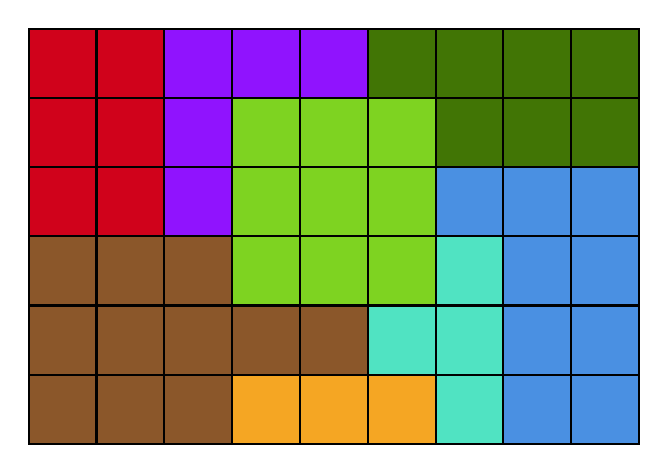
\begin{tikzpicture}[x=1pt,y=1pt,yscale=-1,scale=2.5]
%uncomment if require: \path (0,235); %set diagram left start at 0, and has height of 235

%Shape: Rectangle [id:dp9777322586147241]
\draw  [color={rgb, 255:red, 0; green, 0; blue, 0 }  ,draw opacity=1 ][fill={rgb, 255:red, 126; green, 211; blue, 33 }  ,fill opacity=1 ][line width=0.75]  (283.48,134.04) -- (293.28,134.04) -- (293.28,144.04) -- (283.48,144.04) -- cycle ;
%Shape: Rectangle [id:dp5643921503512281]
\draw  [color={rgb, 255:red, 0; green, 0; blue, 0 }  ,draw opacity=1 ][fill={rgb, 255:red, 126; green, 211; blue, 33 }  ,fill opacity=1 ][line width=0.75]  (293.28,134.04) -- (303.08,134.04) -- (303.08,144.04) -- (293.28,144.04) -- cycle ;
%Shape: Rectangle [id:dp2656365377183654]
\draw  [color={rgb, 255:red, 0; green, 0; blue, 0 }  ,draw opacity=1 ][fill={rgb, 255:red, 126; green, 211; blue, 33 }  ,fill opacity=1 ][line width=0.75]  (283.48,144.04) -- (293.28,144.04) -- (293.28,154.04) -- (283.48,154.04) -- cycle ;
%Shape: Rectangle [id:dp3442854146601232]
\draw  [color={rgb, 255:red, 0; green, 0; blue, 0 }  ,draw opacity=1 ][fill={rgb, 255:red, 126; green, 211; blue, 33 }  ,fill opacity=1 ][line width=0.75]  (293.28,144.04) -- (303.08,144.04) -- (303.08,154.04) -- (293.28,154.04) -- cycle ;
%Shape: Rectangle [id:dp026943086469769284]
\draw  [color={rgb, 255:red, 0; green, 0; blue, 0 }  ,draw opacity=1 ][fill={rgb, 255:red, 126; green, 211; blue, 33 }  ,fill opacity=1 ][line width=0.75]  (303.08,134.04) -- (312.88,134.04) -- (312.88,144.04) -- (303.08,144.04) -- cycle ;
%Shape: Rectangle [id:dp24178310152356564]
\draw  [color={rgb, 255:red, 0; green, 0; blue, 0 }  ,draw opacity=1 ][fill={rgb, 255:red, 126; green, 211; blue, 33 }  ,fill opacity=1 ][line width=0.75]  (303.08,144.04) -- (312.88,144.04) -- (312.88,154.04) -- (303.08,154.04) -- cycle ;
%Shape: Rectangle [id:dp8978302733140608]
\draw  [color={rgb, 255:red, 0; green, 0; blue, 0 }  ,draw opacity=1 ][fill={rgb, 255:red, 126; green, 211; blue, 33 }  ,fill opacity=1 ][line width=0.75]  (303.08,154.04) -- (312.88,154.04) -- (312.88,164.04) -- (303.08,164.04) -- cycle ;
%Shape: Rectangle [id:dp9781999160020896]
\draw  [color={rgb, 255:red, 0; green, 0; blue, 0 }  ,draw opacity=1 ][fill={rgb, 255:red, 126; green, 211; blue, 33 }  ,fill opacity=1 ][line width=0.75]  (293.28,154.04) -- (303.08,154.04) -- (303.08,164.04) -- (293.28,164.04) -- cycle ;
%Shape: Rectangle [id:dp9948264741762237]
\draw  [color={rgb, 255:red, 0; green, 0; blue, 0 }  ,draw opacity=1 ][fill={rgb, 255:red, 126; green, 211; blue, 33 }  ,fill opacity=1 ][line width=0.75]  (283.48,154.04) -- (293.28,154.04) -- (293.28,164.04) -- (283.48,164.04) -- cycle ;
%Shape: Rectangle [id:dp7670141233033437]
\draw  [color={rgb, 255:red, 0; green, 0; blue, 0 }  ,draw opacity=1 ][fill={rgb, 255:red, 245; green, 166; blue, 35 }  ,fill opacity=1 ][line width=0.75]  (303.08,174.04) -- (312.88,174.04) -- (312.88,184.04) -- (303.08,184.04) -- cycle ;
%Shape: Rectangle [id:dp04088026261938915]
\draw  [color={rgb, 255:red, 0; green, 0; blue, 0 }  ,draw opacity=1 ][fill={rgb, 255:red, 245; green, 166; blue, 35 }  ,fill opacity=1 ][line width=0.75]  (293.28,174.04) -- (303.08,174.04) -- (303.08,184.04) -- (293.28,184.04) -- cycle ;
%Shape: Rectangle [id:dp23910333841895082]
\draw  [color={rgb, 255:red, 0; green, 0; blue, 0 }  ,draw opacity=1 ][fill={rgb, 255:red, 245; green, 166; blue, 35 }  ,fill opacity=1 ][line width=0.75]  (283.48,174.04) -- (293.28,174.04) -- (293.28,184.04) -- (283.48,184.04) -- cycle ;
%Shape: Rectangle [id:dp5479449658889934]
\draw  [color={rgb, 255:red, 0; green, 0; blue, 0 }  ,draw opacity=1 ][fill={rgb, 255:red, 80; green, 227; blue, 194 }  ,fill opacity=1 ][line width=0.75]  (312.88,164.04) -- (322.68,164.04) -- (322.68,174.04) -- (312.88,174.04) -- cycle ;
%Shape: Rectangle [id:dp24900658665942066]
\draw  [color={rgb, 255:red, 0; green, 0; blue, 0 }  ,draw opacity=1 ][fill={rgb, 255:red, 80; green, 227; blue, 194 }  ,fill opacity=1 ][line width=0.75]  (312.88,174.04) -- (322.68,174.04) -- (322.68,184.04) -- (312.88,184.04) -- cycle ;
%Shape: Rectangle [id:dp9051424246072522]
\draw  [color={rgb, 255:red, 0; green, 0; blue, 0 }  ,draw opacity=1 ][fill={rgb, 255:red, 80; green, 227; blue, 194 }  ,fill opacity=1 ][line width=0.75]  (312.88,154.04) -- (322.68,154.04) -- (322.68,164.04) -- (312.88,164.04) -- cycle ;
%Shape: Rectangle [id:dp20877566400813574]
\draw  [color={rgb, 255:red, 0; green, 0; blue, 0 }  ,draw opacity=1 ][fill={rgb, 255:red, 80; green, 227; blue, 194 }  ,fill opacity=1 ][line width=0.75]  (303.08,164.04) -- (312.88,164.04) -- (312.88,174.04) -- (303.08,174.04) -- cycle ;
%Shape: Rectangle [id:dp7463070383085549]
\draw  [color={rgb, 255:red, 0; green, 0; blue, 0 }  ,draw opacity=1 ][fill={rgb, 255:red, 144; green, 19; blue, 254 }  ,fill opacity=1 ][line width=0.75]  (273.68,134.04) -- (283.48,134.04) -- (283.48,144.04) -- (273.68,144.04) -- cycle ;
%Shape: Rectangle [id:dp5817482651613091]
\draw  [color={rgb, 255:red, 0; green, 0; blue, 0 }  ,draw opacity=1 ][fill={rgb, 255:red, 144; green, 19; blue, 254 }  ,fill opacity=1 ][line width=0.75]  (273.68,124.04) -- (283.48,124.04) -- (283.48,134.04) -- (273.68,134.04) -- cycle ;
%Shape: Rectangle [id:dp5139194366611862]
\draw  [color={rgb, 255:red, 0; green, 0; blue, 0 }  ,draw opacity=1 ][fill={rgb, 255:red, 144; green, 19; blue, 254 }  ,fill opacity=1 ][line width=0.75]  (273.68,144.04) -- (283.48,144.04) -- (283.48,154.04) -- (273.68,154.04) -- cycle ;
%Shape: Rectangle [id:dp0844836236320533]
\draw  [color={rgb, 255:red, 0; green, 0; blue, 0 }  ,draw opacity=1 ][fill={rgb, 255:red, 144; green, 19; blue, 254 }  ,fill opacity=1 ][line width=0.75]  (283.48,124.04) -- (293.28,124.04) -- (293.28,134.04) -- (283.48,134.04) -- cycle ;
%Shape: Rectangle [id:dp6981612904215215]
\draw  [color={rgb, 255:red, 0; green, 0; blue, 0 }  ,draw opacity=1 ][fill={rgb, 255:red, 144; green, 19; blue, 254 }  ,fill opacity=1 ][line width=0.75]  (293.28,124.04) -- (303.08,124.04) -- (303.08,134.04) -- (293.28,134.04) -- cycle ;
%Shape: Rectangle [id:dp5551743492475295]
\draw  [color={rgb, 255:red, 0; green, 0; blue, 0 }  ,draw opacity=1 ][fill={rgb, 255:red, 139; green, 87; blue, 42 }  ,fill opacity=1 ][line width=0.75]  (254.08,154.04) -- (263.88,154.04) -- (263.88,164.04) -- (254.08,164.04) -- cycle ;
%Shape: Rectangle [id:dp5756209184456107]
\draw  [color={rgb, 255:red, 0; green, 0; blue, 0 }  ,draw opacity=1 ][fill={rgb, 255:red, 139; green, 87; blue, 42 }  ,fill opacity=1 ][line width=0.75]  (254.08,164.04) -- (263.88,164.04) -- (263.88,174.04) -- (254.08,174.04) -- cycle ;
%Shape: Rectangle [id:dp6348941330811271]
\draw  [color={rgb, 255:red, 0; green, 0; blue, 0 }  ,draw opacity=1 ][fill={rgb, 255:red, 139; green, 87; blue, 42 }  ,fill opacity=1 ][line width=0.75]  (263.88,154.04) -- (273.68,154.04) -- (273.68,164.04) -- (263.88,164.04) -- cycle ;
%Shape: Rectangle [id:dp8301788734565072]
\draw  [color={rgb, 255:red, 0; green, 0; blue, 0 }  ,draw opacity=1 ][fill={rgb, 255:red, 139; green, 87; blue, 42 }  ,fill opacity=1 ][line width=0.75]  (263.88,164.04) -- (273.68,164.04) -- (273.68,174.04) -- (263.88,174.04) -- cycle ;
%Shape: Rectangle [id:dp7829057338389512]
\draw  [color={rgb, 255:red, 0; green, 0; blue, 0 }  ,draw opacity=1 ][fill={rgb, 255:red, 139; green, 87; blue, 42 }  ,fill opacity=1 ][line width=0.75]  (254.08,174.04) -- (263.88,174.04) -- (263.88,184.04) -- (254.08,184.04) -- cycle ;
%Shape: Rectangle [id:dp3712039551146994]
\draw  [color={rgb, 255:red, 0; green, 0; blue, 0 }  ,draw opacity=1 ][fill={rgb, 255:red, 139; green, 87; blue, 42 }  ,fill opacity=1 ][line width=0.75]  (263.88,174.04) -- (273.68,174.04) -- (273.68,184.04) -- (263.88,184.04) -- cycle ;
%Shape: Rectangle [id:dp13285358475192177]
\draw  [color={rgb, 255:red, 0; green, 0; blue, 0 }  ,draw opacity=1 ][fill={rgb, 255:red, 139; green, 87; blue, 42 }  ,fill opacity=1 ][line width=0.75]  (273.68,174.04) -- (283.48,174.04) -- (283.48,184.04) -- (273.68,184.04) -- cycle ;
%Shape: Rectangle [id:dp7715824790936205]
\draw  [color={rgb, 255:red, 0; green, 0; blue, 0 }  ,draw opacity=1 ][fill={rgb, 255:red, 139; green, 87; blue, 42 }  ,fill opacity=1 ][line width=0.75]  (273.68,164.04) -- (283.48,164.04) -- (283.48,174.04) -- (273.68,174.04) -- cycle ;
%Shape: Rectangle [id:dp3449796101141618]
\draw  [color={rgb, 255:red, 0; green, 0; blue, 0 }  ,draw opacity=1 ][fill={rgb, 255:red, 139; green, 87; blue, 42 }  ,fill opacity=1 ][line width=0.75]  (273.68,154.04) -- (283.48,154.04) -- (283.48,164.04) -- (273.68,164.04) -- cycle ;
%Shape: Rectangle [id:dp16677713737745214]
\draw  [color={rgb, 255:red, 0; green, 0; blue, 0 }  ,draw opacity=1 ][fill={rgb, 255:red, 139; green, 87; blue, 42 }  ,fill opacity=1 ][line width=0.75]  (293.28,164.04) -- (303.08,164.04) -- (303.08,174.04) -- (293.28,174.04) -- cycle ;
%Shape: Rectangle [id:dp2763666458417998]
\draw  [color={rgb, 255:red, 0; green, 0; blue, 0 }  ,draw opacity=1 ][fill={rgb, 255:red, 139; green, 87; blue, 42 }  ,fill opacity=1 ][line width=0.75]  (283.48,164.04) -- (293.28,164.04) -- (293.28,174.04) -- (283.48,174.04) -- cycle ;
%Shape: Rectangle [id:dp8168324856584601]
\draw  [color={rgb, 255:red, 0; green, 0; blue, 0 }  ,draw opacity=1 ][fill={rgb, 255:red, 208; green, 2; blue, 27 }  ,fill opacity=1 ][line width=0.75]  (254.08,124.04) -- (263.88,124.04) -- (263.88,134.04) -- (254.08,134.04) -- cycle ;
%Shape: Rectangle [id:dp7214289647668896]
\draw  [color={rgb, 255:red, 0; green, 0; blue, 0 }  ,draw opacity=1 ][fill={rgb, 255:red, 208; green, 2; blue, 27 }  ,fill opacity=1 ][line width=0.75]  (254.08,134.04) -- (263.88,134.04) -- (263.88,144.04) -- (254.08,144.04) -- cycle ;
%Shape: Rectangle [id:dp2259114419872651]
\draw  [color={rgb, 255:red, 0; green, 0; blue, 0 }  ,draw opacity=1 ][fill={rgb, 255:red, 208; green, 2; blue, 27 }  ,fill opacity=1 ][line width=0.75]  (263.88,134.04) -- (273.68,134.04) -- (273.68,144.04) -- (263.88,144.04) -- cycle ;
%Shape: Rectangle [id:dp4717862997923473]
\draw  [color={rgb, 255:red, 0; green, 0; blue, 0 }  ,draw opacity=1 ][fill={rgb, 255:red, 208; green, 2; blue, 27 }  ,fill opacity=1 ][line width=0.75]  (254.08,144.04) -- (263.88,144.04) -- (263.88,154.04) -- (254.08,154.04) -- cycle ;
%Shape: Rectangle [id:dp9611478122162561]
\draw  [color={rgb, 255:red, 0; green, 0; blue, 0 }  ,draw opacity=1 ][fill={rgb, 255:red, 208; green, 2; blue, 27 }  ,fill opacity=1 ][line width=0.75]  (263.88,124.04) -- (273.68,124.04) -- (273.68,134.04) -- (263.88,134.04) -- cycle ;
%Shape: Rectangle [id:dp7494245037857424]
\draw  [color={rgb, 255:red, 0; green, 0; blue, 0 }  ,draw opacity=1 ][fill={rgb, 255:red, 208; green, 2; blue, 27 }  ,fill opacity=1 ][line width=0.75]  (263.88,144.04) -- (273.68,144.04) -- (273.68,154.04) -- (263.88,154.04) -- cycle ;
%Shape: Rectangle [id:dp6232296167130805]
\draw  [color={rgb, 255:red, 0; green, 0; blue, 0 }  ,draw opacity=1 ][fill={rgb, 255:red, 74; green, 144; blue, 226 }  ,fill opacity=1 ][line width=0.75]  (322.68,174.04) -- (332.48,174.04) -- (332.48,184.04) -- (322.68,184.04) -- cycle ;
%Shape: Rectangle [id:dp8683869337578874]
\draw  [color={rgb, 255:red, 0; green, 0; blue, 0 }  ,draw opacity=1 ][fill={rgb, 255:red, 74; green, 144; blue, 226 }  ,fill opacity=1 ][line width=0.75]  (332.48,164.04) -- (342.28,164.04) -- (342.28,174.04) -- (332.48,174.04) -- cycle ;
%Shape: Rectangle [id:dp7124076163428046]
\draw  [color={rgb, 255:red, 0; green, 0; blue, 0 }  ,draw opacity=1 ][fill={rgb, 255:red, 74; green, 144; blue, 226 }  ,fill opacity=1 ][line width=0.75]  (332.48,174.04) -- (342.28,174.04) -- (342.28,184.04) -- (332.48,184.04) -- cycle ;
%Shape: Rectangle [id:dp6456653335371463]
\draw  [color={rgb, 255:red, 0; green, 0; blue, 0 }  ,draw opacity=1 ][fill={rgb, 255:red, 74; green, 144; blue, 226 }  ,fill opacity=1 ][line width=0.75]  (332.48,154.04) -- (342.28,154.04) -- (342.28,164.04) -- (332.48,164.04) -- cycle ;
%Shape: Rectangle [id:dp7585326477718629]
\draw  [color={rgb, 255:red, 0; green, 0; blue, 0 }  ,draw opacity=1 ][fill={rgb, 255:red, 74; green, 144; blue, 226 }  ,fill opacity=1 ][line width=0.75]  (332.48,144.04) -- (342.28,144.04) -- (342.28,154.04) -- (332.48,154.04) -- cycle ;
%Shape: Rectangle [id:dp6160757259731467]
\draw  [color={rgb, 255:red, 0; green, 0; blue, 0 }  ,draw opacity=1 ][fill={rgb, 255:red, 74; green, 144; blue, 226 }  ,fill opacity=1 ][line width=0.75]  (322.68,144.04) -- (332.48,144.04) -- (332.48,154.04) -- (322.68,154.04) -- cycle ;
%Shape: Rectangle [id:dp006474296055878126]
\draw  [color={rgb, 255:red, 0; green, 0; blue, 0 }  ,draw opacity=1 ][fill={rgb, 255:red, 74; green, 144; blue, 226 }  ,fill opacity=1 ][line width=0.75]  (312.88,144.04) -- (322.68,144.04) -- (322.68,154.04) -- (312.88,154.04) -- cycle ;
%Shape: Rectangle [id:dp5090163286459264]
\draw  [color={rgb, 255:red, 0; green, 0; blue, 0 }  ,draw opacity=1 ][fill={rgb, 255:red, 74; green, 144; blue, 226 }  ,fill opacity=1 ][line width=0.75]  (322.68,154.04) -- (332.48,154.04) -- (332.48,164.04) -- (322.68,164.04) -- cycle ;
%Shape: Rectangle [id:dp906789860877004]
\draw  [color={rgb, 255:red, 0; green, 0; blue, 0 }  ,draw opacity=1 ][fill={rgb, 255:red, 74; green, 144; blue, 226 }  ,fill opacity=1 ][line width=0.75]  (322.68,164.04) -- (332.48,164.04) -- (332.48,174.04) -- (322.68,174.04) -- cycle ;
%Shape: Rectangle [id:dp6011585657537859]
\draw  [color={rgb, 255:red, 0; green, 0; blue, 0 }  ,draw opacity=1 ][fill={rgb, 255:red, 65; green, 117; blue, 5 }  ,fill opacity=1 ][line width=0.75]  (312.88,124.04) -- (322.68,124.04) -- (322.68,134.04) -- (312.88,134.04) -- cycle ;
%Shape: Rectangle [id:dp41702289164611983]
\draw  [color={rgb, 255:red, 0; green, 0; blue, 0 }  ,draw opacity=1 ][fill={rgb, 255:red, 65; green, 117; blue, 5 }  ,fill opacity=1 ][line width=0.75]  (303.08,124.04) -- (312.88,124.04) -- (312.88,134.04) -- (303.08,134.04) -- cycle ;
%Shape: Rectangle [id:dp7475521297203958]
\draw  [color={rgb, 255:red, 0; green, 0; blue, 0 }  ,draw opacity=1 ][fill={rgb, 255:red, 65; green, 117; blue, 5 }  ,fill opacity=1 ][line width=0.75]  (312.88,134.04) -- (322.68,134.04) -- (322.68,144.04) -- (312.88,144.04) -- cycle ;
%Shape: Rectangle [id:dp7415821682894657]
\draw  [color={rgb, 255:red, 0; green, 0; blue, 0 }  ,draw opacity=1 ][fill={rgb, 255:red, 65; green, 117; blue, 5 }  ,fill opacity=1 ][line width=0.75]  (322.68,134.04) -- (332.48,134.04) -- (332.48,144.04) -- (322.68,144.04) -- cycle ;
%Shape: Rectangle [id:dp12102946712408946]
\draw  [color={rgb, 255:red, 0; green, 0; blue, 0 }  ,draw opacity=1 ][fill={rgb, 255:red, 65; green, 117; blue, 5 }  ,fill opacity=1 ][line width=0.75]  (332.48,134.04) -- (342.28,134.04) -- (342.28,144.04) -- (332.48,144.04) -- cycle ;
%Shape: Rectangle [id:dp026773285156175275]
\draw  [color={rgb, 255:red, 0; green, 0; blue, 0 }  ,draw opacity=1 ][fill={rgb, 255:red, 65; green, 117; blue, 5 }  ,fill opacity=1 ][line width=0.75]  (332.48,124.04) -- (342.28,124.04) -- (342.28,134.04) -- (332.48,134.04) -- cycle ;
%Shape: Rectangle [id:dp7362798318979569]
\draw  [color={rgb, 255:red, 0; green, 0; blue, 0 }  ,draw opacity=1 ][fill={rgb, 255:red, 65; green, 117; blue, 5 }  ,fill opacity=1 ][line width=0.75]  (322.68,124.04) -- (332.48,124.04) -- (332.48,134.04) -- (322.68,134.04) -- cycle ;
\end{tikzpicture}

\end{center}
\caption{Disposición solución de los objetos en la maleta}
\end{figure}

Se pide elaborar un algoritmo de exploración de grafos que resuelva este problema.

\pagebreak

\section{Análisis del problema}\label{grafos-analisis}

Antes de abordar el problema parece sensato realizar una simplificación sobre el mismo:

Las piezas que componen el problema se definen como rectándulos de $5\times5$ casillas.
Sin embargo, un vistazo rápido a las piezas nos da dos formas de simplificar enormemente el ejercicio:

\begin{itemize}
	\item\textbf{No todas las piezas son rectángulos:} Ya que las piezas deberán rotarse para encontrar su solución (como ocurre con la $T$ aguamarina o la pieza marrón), podemos diferenciar entre piezas con una, dos y cuatro rotaciones:
	\begin{itemize}
		\item\textbf{Una rotación:} La pieza es un cuadrado y sus rotaciones resultan en la misma forma que la original. La única que cumple esto es el cuadrado $3\times3$ de color verde claro.
		\item\textbf{Dos rotaciones:} La pieza es un rectángulo y sus rotaciones están emparejadas en función de la relación de orden entre la base y la altura. Cumplen esta condición la $I$ naranja y el rectángulo rojo oscuro.
		\item\textbf{Cuatro rotaciones:} La pieza es irregular y cada rotación se distingue perfectamente de las anteriores.
	\end{itemize}
	\item\textbf{El espacio vacío resultante de definir las piezas como rectángulos $\boldsymbol{5\times5}$ es redundante:} Por ello, definiremos las piezas cada una con una $altura$ y $anchura$ determinadas. De esta forma, la implementación del algoritmo resultará mucho más sencilla.
\end{itemize}

Trabajando en términos numéricos, podemos definir la posición de cada pieza como un vector de tres dimensiones:

\[\text{Posición final} = \big(x,y,rotaci\acute{o}n\big)\]

Tenemos que cada pieza se coloca en una casilla del eje $x$ y una casilla del eje $y$ y toma una $rotaci\acute{o}n\in\mathbb{N}:rotaci\acute{o}n<4$.
Con estos datos, podemos organizar las ocho piezas con las que trabajamos (o el número que fuesen en cualquier otro caso) y ordenar sus posiciones finales en una matriz $n\times3$ para $n$ piezas.
En caso de que la matriz tenga una solución, ésta será una disposición de los valores que forman la posición final de cada una de las piezas, por lo que una solución trivial pero altamente inefectiva del problema será probar una a una y en orden todas las posibles combinaciones de valores que podrían formar una solución, sobre todo teniendo en cuenta que trabajamos con un número discreto de valores, ya que el dominio de los valores solución es $\mathbb{N}$.

Demostrado que podemos resolver el ejercicio por fuerza bruta, procedemos a formular una búsqueda de la solución más eficiente y elegante.
Se tiene que una forma de ordenar las soluciones al problema es mediante un árbol de $n$ niveles para $n$ piezas
El nivel $0$ contendrá todos los elementos inicializados a valores nulos, el primero, todas las combinaciones de valores posibles para la primera pieza y, recursivamente, cada nivel $i$ contendrá todas las combinaciones posibles de la pieza $p_i$ junto con la combinación de la pieza $p_{i-1}$ del nodo padre.

\begin{center}
\tikzset{level distance = 50pt}
\begin{tikzpicture}[grow'=down]
\Tree
[.$\big[\ \ \big]$
		$\big[(5,8,3)\big]$
		$\big[(5,8,2)\big]$
		$\cdots$
		$\big[(0,1,0)\big]$
		[.$\big[(0,0,3)\big]$
			$\big[(0,1,0),(0,0,1)\big]$
			$\big[(0,1,0),(0,0,0)\big]$
		]
		$\big[(0,0,2)\big]$
		$\big[(0,0,1)\big]$
		$\big[(0,0,0)\big]$
	]
\end{tikzpicture}
\end{center}

Recorriendo este árbol podemos encontrar una solución navegando hasta las hojas y reconstruyendo el tablero con ellas.
Sabremos que hemos encontrado la solución si la configuración descrita por la hoja no deja ningún espacio del tablero desocoupado.

Tal y como se plantea el ejercicio, cada nodo de este árbol tiene $6\cdot9\cdot4=216$ hijos, y $8$ niveles, por lo que deberemos comprobar $216^8=4738381338321616896$ diferentes candidatos a soluciones.
Dado que este valor, por muy gestionable que pueda resultar, no permite encontrar una solución en un tiempo admisible, procedemos a definir una serie de podas que realizamos sobre el mismo:

\begin{itemize}
	\item\textbf{Piezas colocadas sobre otras:} Ésta es la poda más obvia de todas. Dado que estamos trabajando en un tablero bidimensional, no podemos colocar piezas sobre otras ni sobreescribir las ya colocadas, por lo que cualquier hijo que intente colocar una pieza sobre otra será automáticamente descartado.
	\item\textbf{Piezas colocadas más allá de los límites del tablero:} El espacio sobre el que trabajamos es limitado. Cualquier pieza colocada de forma que uno de sus componentes se posicionen fuera de los límites del tablero será descartada automáticamente.
	\item\textbf{Piezas cuadradas o rectangulares:} Se eliminan las rotaciones redundantes expuestas en \S\ref{grafos-analisis}.
	\item\textbf{Piezas que, al colocarse, dejan \textit{huecos} en los que no se pueden colocar otras piezas:} En este caso, no tiene sentido seguir probando soluciones descendientes, ya que nunca encontraremos una solución válida.
\end{itemize}

Para esta última poda debemos definir con qué términos vamos a trabajar para tomar esta decisión.
Dado el conjunto de piezas $P$, definimos el tamaño $t(p)$ de una pieza $p$ como su número de componentes.
Tomando como ejemplo las piezas mostradas en \S\ref{grafos-enunciado}, el cuadrado verde tiene un tamaño de $9$ mientras que la $T$ aguamarina tiene un tamaño de $4$.
Por otro lado, definimos el total de casillas accesibles $c_a$ de una casilla $c$ como el número de casillas vacías distintas a las que se puede viajar desde $c$ mediante saltos a las casillas ortogonalmente colindantes.

De esta forma, podemos afirmar que el puzle será irresoluble si $\exists c_a:c_a<\min(t(p_i)),\forall p\in P$.
En la práctica tomaremos estos valores mediante una búsqueda en profundidad (\code{DFS}), de forma que $\min(t(p_i)),\forall p\in P$ valdrá $54$ para la configuración inicial del puzle propuesto en \S\ref{grafos-enunciado} y $0$ o un valor nulo cuando todas las piezas estén colocadas correctamente.

\section{Diseño del algoritmo}\label{grafos-algoritmo}

\subsection{Definiciones del modelo}\label{grafos-algoritmo-definiciones}

Para el diseño de este algoritmo definimos primero qué compone y qué operaciones pueden realizarse sobre las piezas y el tablero.

\subsubsection{Pieza}\label{grafos-algoritmo-definiciones-pieza}

Definimos una pieza como una matriz $h\times b$ en la que cada elemento puede identificarse booleanamente como \code{true} si se corresponde con un componente del modelo o como \code{false} si se corresponde con un espacio vacío.

Las piezas tienen las siguientes características:

\begin{itemize}
	\item\textbf{Altura:} Valor $h$ de la matriz.
	\item\textbf{Anchura:} Valor $b$ de la matriz.
	\item\textbf{Tamaño:} Total de elementos \code{true} de la matriz.
\end{itemize}

Podemos realizar las siguientes operaciones sobre una pieza:

\begin{itemize}
	\item\textbf{Colocar:} Para cada uno de los componentes de la pieza, identificados por un vector bidimensional $(x,y)$, se comprueba que cada componente se corresponda con una casilla vacía equidistante del origen en el tablero. Se considera que la pieza está colocada únicamente si todos los componentes se corresponden con una casilla vacía.
	\item\textbf{Rotar:} Dada una pieza encapsulada en un rectángulo de tamaño $h\times b$, se realiza una rotación de $90^{\circ}$, $180^{\circ}$ o $270^{\circ}$, de forma que el tamaño de la pieza pasa a ser $b\times h$, $-h\times-b$ y $-b\times-h$, respectivamente. Tras esta operación, se devuelve el origen a la esquina superior derecha para simplificar los cálculos.
\end{itemize}

\subsubsection{Tablero}\label{grafos-algoritmo-definiciones-tablero}

Definimos el tablero como una matriz $h\times b$ en la que cada elemento puede identificarse booleanamente como \code{true} si una pieza está ocupando su lugar o como \code{false} si se encuentra libre.

El tablero tiene las siguientes características:

\begin{itemize}
	\item\textbf{Altura:} Valor $h$ de la matriz.
	\item\textbf{Anchura:} Valor $b$ de la matriz.
\end{itemize}

Sobre el tablero podemos realizar una búsqueda en profundidad a partir de una de sus casillas para consultar el tamaño del \textit{hueco} en el ésta se encuentra.

\subsection{Estructura del algoritmo}\label{grafos-algoritmo-estructura}

Supuestos inicializados los elementos del modelo como veremos en \S\ref{grafos-implementacion}, definimos el algoritmo como una función recursiva que recorra, para una pieza, todas las posibles posiciones en las que se puede colocar con cada rotación.
En caso de encontrar una posición válida, el algoritmo se llamará a sí mismo indicando que debe probar con una pieza nueva teniendo en cuenta la ya colocada.
Para cada llamada el algoritmo recibe los siguientes argumentos:

\begin{itemize}
	\item El tablero sobre el que se colocan las piezas.
	\item La lista de piezas a colocar.
	\item El índice de la pieza con la que opera.
	\item Condición de resolución del sistema para propagar a los nodos ancestros.
\end{itemize}

Para probar una posición válida, el algoritmo puede almacenar las piezas que ha ido colocando y eliminarlas en cualquier momento o copiar el tablero y probar a colocar la pieza con la copia.
Elegimos la segunda opción porque, a pesar de ser menos eficiente en memoria, resulta más sencilla de implementar.
Siguiendo estos patrones de diseño, el algoritmo quedaría de esta forma:

\subsubsection{Función principal}

\begin{lstlisting}[language=Python]
Algoritmo (tablero, piezas, indice, resuelto)
	for fila in tablero
		for columna in tablero
			for rotacion in rotaciones
				tablero_hijo = tablero

				if Colocar()
					accesibles = tablero.TestAccesibilidad()

					if accesibles != null
						resuelto = accesibles == 0

						if not resuelto and accesibles >= MinimoTamanio(piezas, indice+1)
							inicio_hijo = indice
							Algoritmo (tablero_hijo, piezas, indice_hijo, resuelto)
\end{lstlisting}

Este algoritmo llama a las siguientes funciones auxiliares:

\begin{itemize}
	\item\code{Colocar}\textbf{:} Intenta colocar una pieza en el tablero y devuelve un valor booleano correspondiente al éxito de la operación.
	\item\code{TestAccesibilidad}\textbf{:} Devuelve el menor valor de casillas accesibles distinto de $0$ en todo el tablero.
	\item\code{MinimoTamanio}\textbf{:} Devuelve el tamaño mínimo de las piezas a partir del índice indicado.
\end{itemize}

Dado que el comportamiento de estas funciones depende del modelo sobre el cual se implementen, dejamos los detalles de su implementación para el siguiente punto.

\section{Implementación del algoritmo}\label{grafos-implementacion}

Para este problema vamos a crear las clases \code{Pieza} y \code{Tablero} y desarrollar el algoritmo sobre ellas.
Mostramos aquí sus prototipos:

\subsection{Clase \code{Pieza}}\label{grafos-implementacion-pieza}

\begin{lstlisting}[language=C++]
class Pieza {
private:
	bool cuadrado,
	     rectangulo;
	char id;

	std::vector<std::vector<bool> > forma;
	std::vector<std::vector<bool> > forma_cw;
	std::vector<std::vector<bool> > forma_ccw;
	std::vector<std::vector<bool> > forma_pi;

	//void Simplifica (std::vector<std::vector<bool> > & forma);
	std::vector<std::vector<bool> > RotaCW  () const;
	std::vector<std::vector<bool> > RotaCW  (const std::vector<std::vector<bool> > & rotable) const;
	std::vector<std::vector<bool> > RotaCCW () const;
	std::vector<std::vector<bool> > RotaPI  () const;

public:
	Pieza (bool c, bool r, char i, std::vector<std::vector<bool> > f);

	size_t Altura     (Rotacion rotacion = Rotacion::Original) const;
	size_t Anchura    (Rotacion rotacion = Rotacion::Original) const;
	size_t Tamanio    () const;
	bool   Cuadrado   () const;
	bool   Rectangulo () const;
	char   ID         () const;

	std::vector<std::vector<bool> > Forma (Rotacion rotacion = Rotacion::Original) const;

	void Imprime (Rotacion rotacion = Rotacion::Original) const;

	bool operator < (const Pieza & otra) const;
};
\end{lstlisting}

Para ahorrar tiempo de ejecución con un coste marginal de memoria, incluimos las cuatro rotaciones en los datos privados de la clase, que se generan con sus correspondientes funciones miembro de rotación.
También incluimos en estos datos privados si la pieza es un cuadrado o un rectángulo y su \code{id}, que es un número que la identifica en su representación en el tablero.

En las funciones miembro públicas, aparte de los consultores de sus atributos, se incluyen una función para mostrar por salida estándar la forma de la pieza y un operador \code{<} para ordenar las piezas, como veremos en~\ref{grafos-implementacion-algoritmo}.
Varias de las funciones de esta clase reciben como argumento una rotación proveniente de la clase \code{Rotacion}, que definimos en el siguiente apartado.

\pagebreak

\subsection{Enumerado \code{Rotacion}}\label{grafos-implementacion-rotacion}

\begin{lstlisting}[language=]
enum class Rotacion {
	CW,
	CCW,
	PI,
	Original
};
\end{lstlisting}

Cada uno de estos elementos representan las siguientes rotaciones:

\begin{itemize}
	\item\code{CW}\textbf{:} Rotación de $90^{\circ}$.
	\item\code{CCW}\textbf{:} Rotación de $270^{\circ}$.
	\item\code{PI}\textbf{:} Rotación de $180^{\circ}$.
	\item\code{Original}\textbf{:} Rotación de $0^{\circ}$.
\end{itemize}

\subsection{Clase \code{Tablero}}\label{grafos-implementacion-tablero}

\begin{lstlisting}[language=C++]
class Tablero {
private:
	std::vector<std::vector<char> > matriz;

	size_t DFS (size_t fila, size_t columna, std::vector<std::vector<char> > & matriz) const;

public:
	Tablero (size_t altura, size_t anchura);
	Tablero (const Tablero & otro);

	size_t Altura  () const;
	size_t Anchura () const;
	std::vector<std::vector<char> > Matriz () const;

	size_t Accesibles () const;
	size_t Accesibles (size_t fila, size_t columna) const;
	size_t Coloca     (size_t fila, size_t columna, Pieza pieza, Rotacion rotacion = Rotacion::Original);
	void   Imprime    (bool sobreescribe = false) const;

	Tablero & operator = (const Tablero & otro);
};
\end{lstlisting}

Esta clase contiene una matriz en la que se representa el tablero.
Esta matriz es de \code{char} para poder identificar las piezas que se colocan en cada casilla, de forma que cada pieza se identifica con un carácter alfanumérico y las casillas vacías con el carácter \code{-}.
Aparte de los consultores y una función de impresión, implementa las siguientes funciones miembro:

\pagebreak

\subsubsection{\code{Accesibles}}\label{grafos-implementacion-tablero-accesibles}

\begin{lstlisting}[language=C++]
size_t Tablero :: Accesibles () const {
	size_t minimo_espacio = UINT_MAX;

	for (size_t i=0; i<Altura(); i++)
		for (size_t j=0; j<Anchura(); j++)
			if (matriz[i][j] == '-')
				minimo_espacio = std::min(minimo_espacio, Accesibles(i, j));

	if (minimo_espacio == UINT_MAX)
		minimo_espacio = 0;

	return minimo_espacio;
}

size_t Tablero :: Accesibles (size_t fila, size_t columna) const {
	size_t accesibles;

	if (matriz[fila][columna] == '-') {
		std::vector<std::vector<char> > matriz_busqueda = matriz;
		accesibles = DFS(fila, columna, matriz_busqueda);
	}
	else {
		accesibles = 0;
	}

	return accesibles;
}
\end{lstlisting}

La versión sin argumentos devuelve el valor mínimo de casillas accesibles como se expuso en \S\ref{grafos-analisis} y la versión con argumentos, el valor de cada una de las casillas a las que accede la anterior.
Esta operación se realiza mediante una búsqueda en profundidad.

\subsubsection{\code{DFS}}\label{grafos-implementacion-tablero-dfs}

\begin{lstlisting}[language=C++]
size_t Tablero :: DFS (size_t fila, size_t columna, std::vector<std::vector<char> > & matriz) const {
	size_t contador = (matriz[fila][columna] == 'T') ? 0 : 1;

	matriz[fila][columna] = 'T';

	if (fila+1 < Altura() && matriz[fila+1][columna] == '-' )
		contador += DFS(fila+1, columna, matriz);

	if (fila != 0 && matriz[fila-1][columna] == '-')
		contador += DFS(fila-1, columna, matriz);

	if (columna+1 < Anchura() && matriz[fila][columna+1] == '-')
		contador += DFS(fila, columna+1, matriz);

	if (columna != 0 && matriz[fila][columna-1] == '-')
		contador += DFS(fila, columna-1, matriz);

	return contador;
}
\end{lstlisting}

Esta búsqueda en profundidad (\textit{Depth First Search}) recibe una copia de la matriz como lista de abiertos y va pasándola por referencia a llamadas recursivas para actualizar su lista de cerrados sumando $1$ por cada casilla accesible en la lista de abiertos.

\subsubsection{\code{Coloca}}\label{grafos-implementacion-tablero-coloca}

\begin{lstlisting}[language=C++]
size_t Tablero :: Coloca (size_t fila, size_t columna, Pieza pieza, Rotacion rotacion) {
	size_t minimo_espacio = UINT_MAX;
	bool colocada = true;
	std::vector<std::vector<char> > prueba = matriz;

	for (size_t i=0; i<pieza.Altura(rotacion) && colocada; i++) {
		for (size_t j=0; j<pieza.Anchura(rotacion) && colocada; j++) {
			if ((colocada = fila+i<Altura() && columna+j<Anchura())) {
				if ((colocada = pieza.Forma(rotacion)[i][j] && prueba[fila+i][columna+j] == '-'))
					prueba[fila+i][columna+j] = pieza.ID();
				else
					colocada = !pieza.Forma(rotacion)[i][j];
			}
		}
	}

	if (colocada) {
		matriz         = prueba;
		minimo_espacio = Accesibles();
	}

	return minimo_espacio;
}
\end{lstlisting}

Para colocar una pieza en el tablero, primero clonamos la matriz en una matriz de \code{prueba}, de forma que sólo sobreescribimos la original si conseguimos colocarla.
La colocación se realiza casilla a casilla de forma que se considera colocada si todos los componentes de la pieza se corresponden con una casilla vacía del tablero.
Para agilizar el trabajo del programador, una vez se comprueba que la pieza está correctamente colocada y se sustituye la matriz original por la clonada, se realiza una llamada a \code{Accesibles()} para obtener el \textit{hueco} de menor tamaño que deja la pieza al ser colocada y se devuelve.
De esta forma, podemos aprovechar los cómputos de esta función miembro para determinar si la colocación de la pieza es correcta sin realizar más operaciones.

\subsection{Algoritmo principal}\label{grafos-implementacion-algoritmo}

Para este algoritmo contamos con una función para inicializar las piezas, y tres funciones sobre las que trabajaremos:

\subsubsection{\code{MinimoTamanio}}\label{grafos-implementacion-algoritmo-minimotamanio}

\begin{lstlisting}[language=C++]
size_t MinimoTamanio (const std::vector<Pieza> & piezas, const size_t inicio) {
	size_t minimo_tamanio = UINT_MAX;

	for (size_t i=inicio; i<piezas.size(); i++)
		minimo_tamanio = std::min(minimo_tamanio, piezas[i].Tamanio());

	return minimo_tamanio;
}
\end{lstlisting}

Esta función simplemente devuelve el tamaño mínimo de las piezas del vector \code{piezas} a partir de la posición de \code{inicio} indicada.

\pagebreak

\subsubsection{\code{Resuelve}}\label{grafos-implementacion-algoritmo-resuelve}

\begin{lstlisting}[language=C++]
bool Resuelve (const Tablero & tablero, std::vector<Pieza> & piezas, const size_t & inicio, bool & resuelto) {
	for (size_t fila=0; fila<tablero.Altura() && !resuelto; fila++) {
		for (size_t columna=0; columna<tablero.Anchura() && !resuelto; columna++) {
			Rotacion rotacion;

			for (unsigned i=0; i<4 && !resuelto; i++) {
				switch (i) {
					case 0: rotacion = Rotacion::Original; break;
					case 1: rotacion = Rotacion::CW;       break;
					case 2: rotacion = Rotacion::CCW;      break;
					case 3: rotacion = Rotacion::PI;       break;
				}

				if ((piezas[inicio].Cuadrado() && rotacion == Rotacion::Original)
				||  (piezas[inicio].Rectangulo() && (rotacion == Rotacion::Original || rotacion == Rotacion::CW))
				||  (!piezas[inicio].Cuadrado() && !piezas[inicio].Rectangulo())) {
					Tablero tablero_hijo(tablero);
					size_t accesibles = tablero_hijo.Coloca(fila, columna, piezas[inicio], rotacion);

					tablero_hijo.Imprime(true);

					if (accesibles != UINT_MAX) {
						resuelto = !accesibles;

						if (!resuelto && accesibles >= MinimoTamanio(piezas, inicio+1)) {
							size_t inicio_hijo = inicio + 1;
							Resuelve(tablero_hijo, piezas, inicio_hijo, resuelto);
						}
					}
				}
			}
		}
	}

	return resuelto;
}
\end{lstlisting}

Para cada fila, columna y rotación, creamos un tablero para el nodo hijo del árbol y comprobamos si la rotación es válida en función de la cuadrangularidad o rectangularidad de la pieza de trabajo e intentamos colocarla.
Si, al colocarla, obtenemos un valor de mínimo de casillas accesibles no nulo (\code{UINT\_MAX}), comprobamos que sea mayor que $0$.
En caso positivo, el puzle sigue sin estar resuelto y se llama recursivamente a la función con la nueva pieza de trabajo.
Si no podemos colocar la pieza en ningún caso, se retrocede en el árbol y se prueba con otros valores.
En caso de que el mínimo de casillas accesibles sea $0$, entendemos que el ejercicio está resuelto (sin importar si se han usado todas las piezas) y propagamos la resolución a nodos anteriores para finalizar la ejecución del algoritmo.

El algoritmo muestra en pantalla la resolución del puzle sobreescribiendo una vez por cada pieza que se coloca\footnote{%
	La forma óptima de mostrarlo, sobre todo para ejecuciones largas, es reproduciendo \href{https://www.youtube.com/watch?v=MK6TXMsvgQg}{el tema principal del Show de Benny Hill} de fondo.
},
de forma que la solución es la última configuración que se muestra.

\pagebreak

\subsubsection{\code{main}}\label{grafos-implementacion-algoritmo-main}

\begin{lstlisting}[language=C++]
int main (int argc, char ** argv) {
	Tablero tablero(6, 9);
	bool resuelto = false;
	std::vector<Pieza> piezas = InicializaPiezas();

	tablero.Imprime();

	std::sort(piezas.begin(), piezas.end());
	std::reverse(piezas.begin(), piezas.end());
	std::cout << (Resuelve(tablero, piezas, 0, resuelto) ? "Solución encontrada."
	                                                     : "Solución no encontrada")
	          << std::endl;

	return 0;
}
\end{lstlisting}

Aparte de inicializar el tablero y las piezas, se optimiza enormemente el algoritmo ordenando el vector de \code{piezas} de mayor a menor tamaño de las mismas, reduciendo el factor de ramificación y el tiempo de ejecución con \code{-O3} de $2m\ 32s$ a menos de $1s$\footnote{%
	Estos números suprimen la llamada a la impresión del tablero.
	Sin optimización de compilación ni impresión se consiguen $2s$ con la reordenación del vector y un abandono de la operación pasados $10m$ sin ésta por parte del usuario porque tiene mejores cosas que hacer con su tiempo.
}.

\section{Ejemplo de resolución}\label{grafos-resolucion}

Para compilar y ejecutar el proyecto basta con ejecutar \code{make \&\& bin/maleta}.
Para el puzle propuesto, el algoritmo curiosamente no devuelve la solución propuesta en \S\ref{grafos-enunciado}, sino la siguiente\footnote{%
	Las piezas están numeradas de $0$ a $7$ en el orden en el que se muestran en \S\ref{grafos-enunciado}.
}:

\begin{lstlisting}
444666655
444666655
444622255
347772000
347777000
333111000
Solución encontrada.
\end{lstlisting}
